% !tex root=../main.tex
\section{Example Programs and Experiments}
\label{sec:exampprog}
\subsection{Programs}

We now present a few simple FOPPL programs and discuss both their statistical forms and the results generated via HMC inference. In all the graphical model plots, shaded circles represent \mintinline{clojure}{observe}d parameters, un-shaded circles represent the latent variables, our parameters of interest, and diamonds represent a deterministic statement. 
\subsubsection{Conjugate Gaussian}
The conjugate Gaussian, see figure (\ref{fig:conga}), is a model in which we can analytically calculate the true posterior $p(x | y)$, as the product of two Gaussians is also a Gaussian. For our particular model we \mintinline{clojure}{sample} $x \sim \mathcal{N}(0, 1)$ and we \mintinline{clojure}{observe} $y = 7$, with likelihood $p(y|x) = \mathcal{N}(y | x, 1)$ and we aim to infer the mean of the posterior. The  FOPPL program for figure (\ref{fig:conga}) is as follows:
\inputminted{clojure}{code/conjugategauss.clj}
\begin{figure}[ht]
	\begin{center}
		% model_pca.tex
%
% Copyright (C) 2012 Jaakko Luttinen
%
% The MIT License
%
% See LICENSE file for more details.

% PCA model

%\beginpgfgraphicnamed{model-pca}
%\begin{tikzpicture}
%
%  % Define nodes
%  \node[obs]                               (y) {$y$};
%  \node[latent, above=of y, xshift=-1.2cm] (w) {$\mathbf{w}$};
%  \node[latent, above=of y, xshift=1.2cm]  (x) {$\mathbf{x}$};
%  \node[latent, right=2cm of y]            (t) {$\tau$};
%
%  % Connect the nodes
%  \edge {x,w,t} {y} ; %
%
%  % Plates
%  \plate {yx} {(x)(y)} {$N$} ;
%  \plate {} {(w)(y)(yx.north west)(yx.south west)} {$M$} ;
%
%\end{tikzpicture}
%\endpgfgraphicnamed

%%% Local Variables: 
%%% mode: tex-pdf
%%% TeX-master: "example"
%%% End: % model_pca.tex
%
% Copyright (C) 2012 Jaakko Luttinen
%
% The MIT License
%
% See LICENSE file for more details.

% PCA model

%\beginpgfgraphicnamed{model-pca}
\begin{tikzpicture}

\node[obs](y){$y$};
% Define nodes
\node[latent, above= of y, xshift=0cm]   (x) {$x$}; 

% Connect the nodes
\edge {x} {y} ; %

% Plates
%\plate {yx} {(x)(y)} {$N$} ;
%\plate {} {(w)(y)(yx.north west)(yx.south west)} {$M$} ;

\end{tikzpicture}
%\endpgfgraphicnamed

%%% Local Variables: 
%%% mode: tex-pdf
%%% TeX-master: "example"
%%% End: 
	\end{center}
	\caption{The graphical model for the conjugate Gaussian}
	\label{fig:conga}
\end{figure}
In calculating the joint of the model, we arrive as the following $ p(x|y) \propto p(x,y) = p(x)p(y| x) = \mathcal{N}(\bar{\mu}, \bar{\sigma}^{2})$, where $\bar{\mu} = \left(\frac{\mu_{0}\sigma^{2} + \sigma^{2}_{0}\sum_{i=1}^{n}y_{i}}{\sigma^{2}\sigma^{2}_{0}}\right) \bar{\sigma}^{2}$ and $\bar{\sigma}^{2} = \left(\frac{1}{\sigma^{2}_{0}} + \frac{n}{\sigma^{2}}\right)^{-1} $,  $n$ is the total number of observed datum $y$, $\mu_{0} = 0 $, $\sigma_{0}^{2} = 1$ are the prior mean and variance and $\sigma^{2} = 1.0 $ is the likelihood variance. Thus, the true mean that our model should infer is $\bar{\mu} = 5$. This is indeed the value that we get as can be seen via figures (\ref{fig:plotconj1}-\ref{fig:plotconj3}).
\subsubsection{Conditional If}
\begin{figure}[ht]
	\begin{center}
		% !tex root=/main.tex
\beginpgfgraphicnamed{conif}
\begin{tikzpicture}

% Define nodes
\node[obs, xshift = -2cm]   (y2){$y$};
\node[obs, xshift = 0cm] (y1){$y$};
\node[det, above= of {y1, y2}, xshift = -1cm ]     (if) {if-else} ; % 
\node[latent, above= of if]             (x){$x$};
%\node[latent, above= of y, xshift=0cm]   (true) {$z_{n}$};
%\node[latent, above=of z, xshift=0cm]   (false) {$s$};
%\node[latent, above=of z, xshift=1.2cm]  (b) {$b$};
%\node[obs, above= of z, xshift=-1.2cm]   (x) {$x_{n}$}; 

% Connect the nodes
\edge {x}{if};
\edge [dashed]{if}{y1,y2};

% Plates
%\plate {yx} {(x)(y)} {$N$} ;
%\plate {} {(w)(y)(yx.north west)(yx.south west)} {$M$} ;

\end{tikzpicture}
	\end{center}
	\caption{The graphical model for condition if}
	\label{fig:conif}
\end{figure}
The conditional \mintinline{clojure}{if} statement, see figure (\ref{fig:conif}), is typically challenging to implement for gradient based methods, due to the branching effects that occur at the condition. For trace based samplers, such as importance sampling, this is not a problem as multiple traces are recorded for each path taken. However, in higher dimensions these types of samplers are heavily impaired, which is why we need additional MCMC methods to be able to perform efficiently in higher dimensions. For the purpose of this paper we provide a low dimensional model, so that we can easily visualize the output of our HMC implementation of the conditional program. In a FOPPL we would write a simple conditional \mintinline{clojure}{if} program as follows:\inputminted{clojure}{code/conditionalif.clj}
 In this model, we have a joint distribution of the form $p(x | y) \propto p(x, y) = \mathcal{N}(0,1)\mathcal{N}(y = 1|1,1)^{\mathbb{I}(x > 0)}\mathcal{N}(y = 1|-1,1)^{\mathbb{I}(x < 0)}$, where $\mathbb{I}(\cdot)$ represents the indicator function. The empirical mean that we generate for this model is 0.58 and if you plot the unnormalized joint, the shape is the same, but the density values are of course different, see figures (\ref{fig:plotif1}-\ref{fig:plotif3}). This implies that we can be confident in the results generated by the HMC. For additional verification the same program was run in Anglican \cite{wood2014new} to ensure that it generated the same results. 
% If we are to analytically calculate the mean, we have to look at the case where $x < 0$ and the case where $x>0$. Using the sum rule the evidence can be found by $p(y) = \int p(x,y) dx $, which we analytically calculate to be, $p_{x<0}(y) = -\mathcal{N}(y=1|-1,1)\sqrt{2\pi}$ and for $x>0$ we have  $p_{x>0}(y) = \mathcal{N}(y=1| 1,1)\sqrt{2\pi}$. Thus, by Bayes rule, the full posterior is given as $p(x | y) = \frac{p(y|x)p(x)}{p(y)} = \frac{\mathcal{N}(0,1)\mathcal{N}(y = 1|1,1)^{\mathbb{I}(x > 0)}\mathcal{N}(y = 1|-1,1)^{\mathbb{I}(x < 0)}}{\sqrt{(2\pi)(\mathcal{N}(y = 1|-1,1)^{\mathbb{I}(x < 0)} + \mathcal{N}(y = 1|1,1)^{\mathbb{I}(x > 0)} )}}$ .    
\subsubsection{Linear Regression}
\begin{figure}[ht]
	\begin{center}
		% model_pca.tex
%
% Copyright (C) 2012 Jaakko Luttinen
%
% The MIT License
%
% See LICENSE file for more details.

% PCA model

%\beginpgfgraphicnamed{model-pca}
%\begin{tikzpicture}
%
%  % Define nodes
%  \node[obs]                               (y) {$y$};
%  \node[latent, above=of y, xshift=-1.2cm] (w) {$\mathbf{w}$};
%  \node[latent, above=of y, xshift=1.2cm]  (x) {$\mathbf{x}$};
%  \node[latent, right=2cm of y]            (t) {$\tau$};
%
%  % Connect the nodes
%  \edge {x,w,t} {y} ; %
%
%  % Plates
%  \plate {yx} {(x)(y)} {$N$} ;
%  \plate {} {(w)(y)(yx.north west)(yx.south west)} {$M$} ;
%
%\end{tikzpicture}
%\endpgfgraphicnamed

%%% Local Variables: 
%%% mode: tex-pdf
%%% TeX-master: "example"
%%% End: % model_pca.tex
%
% Copyright (C) 2012 Jaakko Luttinen
%
% The MIT License
%
% See LICENSE file for more details.

% PCA model

%\beginpgfgraphicnamed{model-pca}
\begin{tikzpicture}

\node[obs](y){$y_{n}$};
% Define nodes
\node[latent, above= of y, xshift=0cm]   (z) {$z_{n}$};
\node[latent, above=of z, xshift=0cm]   (s) {$s$};
\node[latent, above=of z, xshift=1.2cm]  (b) {$b$};
\node[obs, above= of z, xshift=-1.2cm]   (x) {$x_{n}$}; 

% Connect the nodes
\edge {x,s,b} {z} ; %
\edge {z} {y} ;

% Plates
%\plate {yx} {(x)(y)} {$N$} ;
%\plate {} {(w)(y)(yx.north west)(yx.south west)} {$M$} ;

\end{tikzpicture}
%\endpgfgraphicnamed

%%% Local Variables: 
%%% mode: tex-pdf
%%% TeX-master: "example"
%%% End: 
	\end{center}
	\caption{The graphical model for Linear regression}
    \label{fig:lrgraph}
\end{figure}
In this problem we have a set of points $\{(x_{n},y_{n})\}$ and we wish to infer the equation of a line in a Bayesian manner, such that the line goes through all of those points. See figure (\ref{fig:lrgraph}) for a graphical model of the model. To do this, we must infer the slope and the bias of the line, which is done by placing priors on our parameters of interest. The FOPPL program corresponding to figure (\ref{fig:lrgraph}) can be written as follows:\inputminted{clojure}{code/linearregression.clj}In this model for both the slope and bias, we \mintinline{clojure}{sample} from $\mathcal{N}(0,10.0)$ and we state that the likelihood of the model is of the form of a conditional Gaussian $\mathcal{N}(y_{n}| z_{n}, 1.0)$ with a mean conditioned on our \mintinline{clojure}{sample}d lines, given the \mintinline{clojure}{observe}d points. Therefore, we can construct the joint for this model as $ p(s,b,z_{n} | x_{n}, y_{n}) \propto p(x_{n},s,b,z_{n}, y_{n}) = p(s)p(b)p(y_{n} | z_{n}, 1) =\mathcal{N}(0,5^{2})\mathcal{N}(y_{n}|z_{n},1.0)$. We can analytically calculate the equation of a straight line by using the formula $\left(\frac{y - y_{*}}{x - x_{*}}\right) = s$, which leads to $y = sx + b$. From which we find that the true slope $s = 1.6$ and the bias $b = 0.5$. We again see from figures (\ref{fig:plotlr1}-\ref{fig:plotlr3}), that the HMC correctly calculates the true values of the parameters.\\

	\begin{figure*}[ht!]
	\centering
	\subcaptionbox{\label{fig:plotconj1}}[.3\linewidth][c]{%
		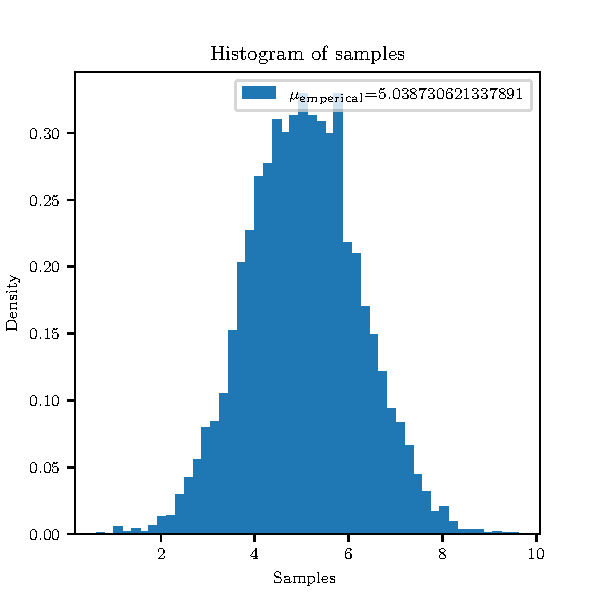
\includegraphics[width=.2\linewidth]{plots/conjgauss/figures/histogram.pdf}}\quad
	\subcaptionbox{}[.3\linewidth][c]{%
		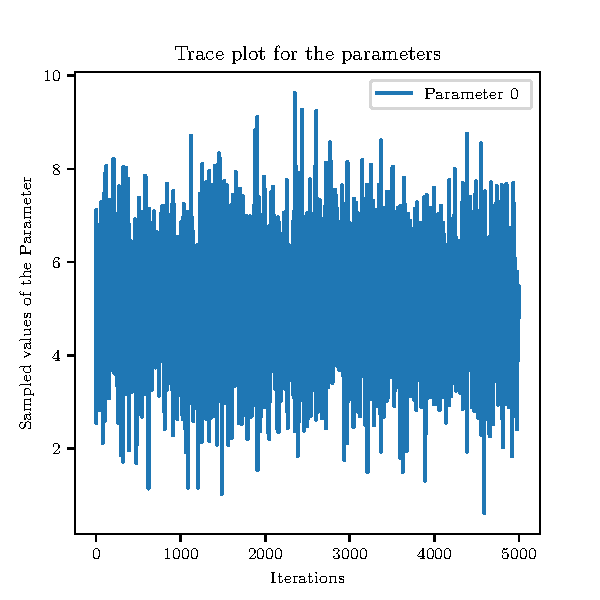
\includegraphics[width=.2\linewidth]{plots/conjgauss/figures/trace.pdf}}\quad
	\subcaptionbox{\label{fig:plotconj3}}[.3\linewidth][c]{%
		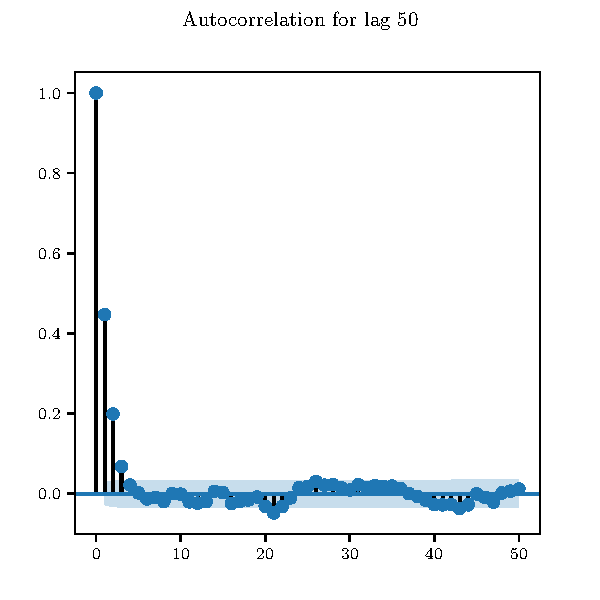
\includegraphics[width=.2\linewidth]{plots/conjgauss/figures/Autocorrelationplot.pdf}}
	
	\bigskip
	\subcaptionbox{	\label{fig:plotif1}}[.3\linewidth][c]{%
		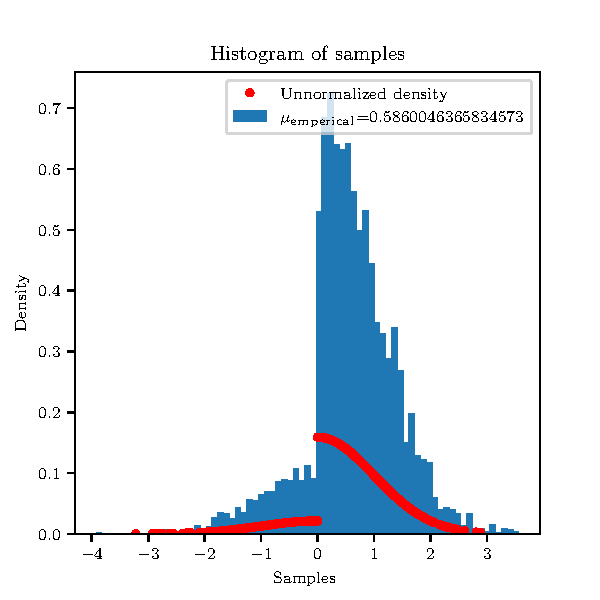
\includegraphics[width=.2\linewidth]{plots/conditionalif/figures/histogramwithdensity.pdf}}\quad
	\subcaptionbox{}[.3\linewidth][c]{%
		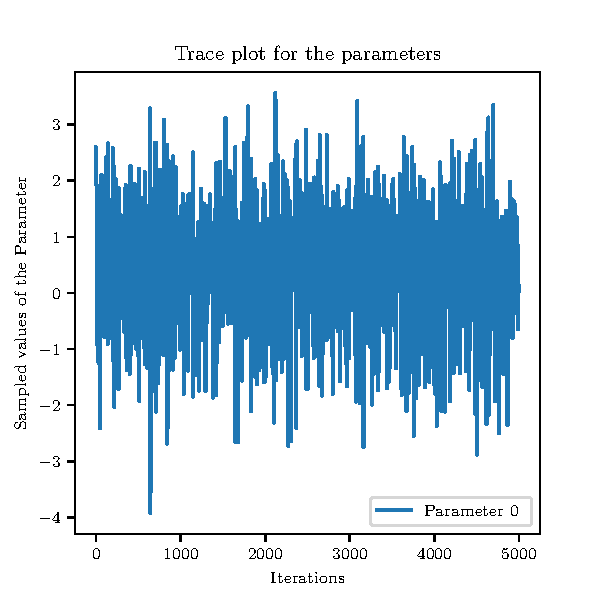
\includegraphics[width=.2\linewidth]{plots/conditionalif/figures/trace.pdf}}\quad
	\subcaptionbox{	\label{fig:plotif3}}[.3\linewidth][c]{%
		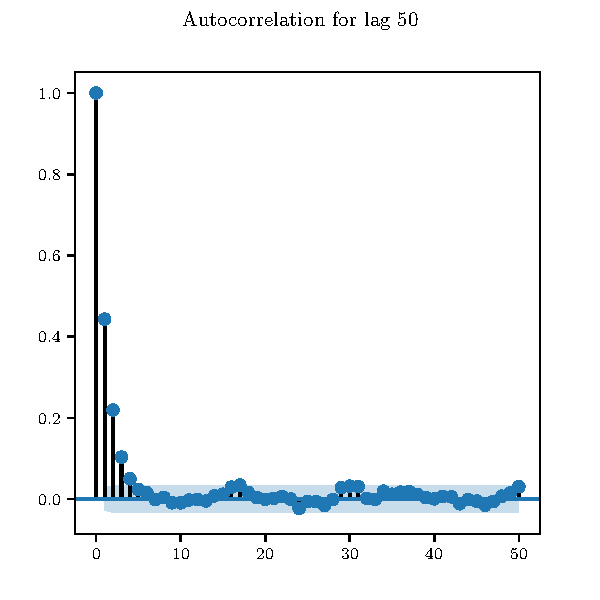
\includegraphics[width=.2\linewidth]{plots/conditionalif/figures/Autocorrelationplot.pdf}}
	
	\bigskip
    \subcaptionbox{	\label{fig:plotlr1} }[.3\linewidth][c]{%
		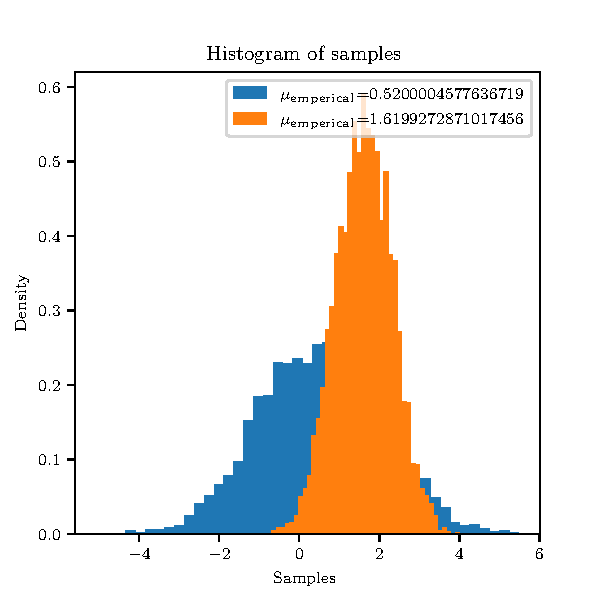
\includegraphics[width=.2\linewidth]{plots/linearreg/figures/histogram.pdf}}\quad
	\subcaptionbox{}[.3\linewidth][c]{%
		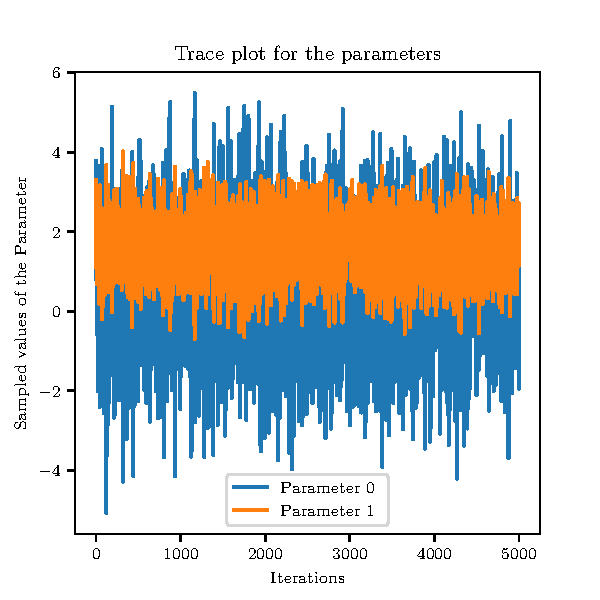
\includegraphics[width=.2\linewidth]{plots/linearreg/figures/trace.pdf}}\quad
	\subcaptionbox{	\label{fig:plotlr3}Left: bias . Right: slope.}[.3\linewidth][c]{%
		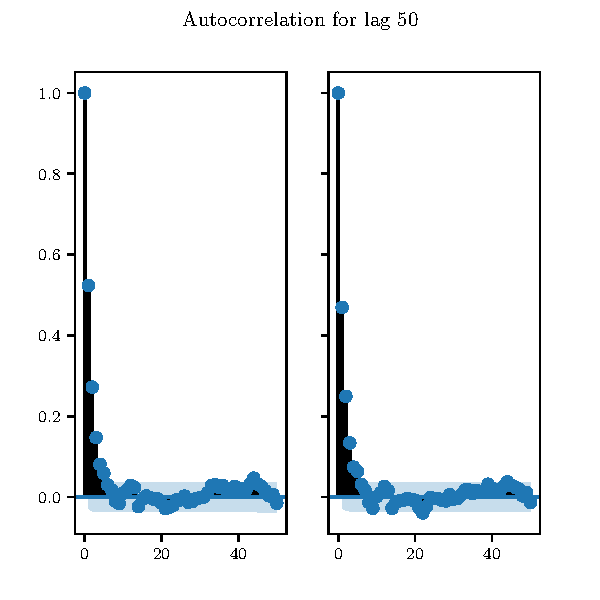
\includegraphics[width=.2\linewidth]{plots/linearreg/figures/Autocorrelationplot.pdf}}
	\caption{Each row corresponds to the inference output of each model and provides a histogram of the samples, the trace of the samples for each parameter of interest in the model and the autocorrelation between the samples for a lag $l = 50$. \textit{Top row} represents the conjugate Gaussian model. \textit{Middle row} represents the conditional if model. \textit{Bottom row} represents the linear regression model with parameter 0, in blue, representing the bias and parameter 1, in orange, representing the slope of the line.  }
	\label{fig:allplots}	
\end{figure*}
\subsection{Experimental Results}
Here we present the results of running HMC inference on our FOPPL programs via the compiled Python output. All plots were generated by running HMC until 1000 samples had been collected, we use no burn in period and so all results presented are of all samples generated. See figure (\ref{fig:allplots}).